%%%%%%%%%%%%%%%%%%%%%%%%%%%%%%%%%%%%%%%%%%%%%%
%                insertmeeting
% 1) Title (something creative & funny?)
% 2) Date (MM/DD/YYYY)
% 3) Location (ex. Hagerty High School)
% 4) People/Committees Present 
% 5) Picture 
% 6) Start Time & Stop Time (ex. 12:30AM to 4:30PM)
%%%%%%%%%%%%%%%%%%%%%%%%%%%%%%%%%%%%%%%%%%%%%%
\insertmeeting 
	{Meeting Example} 
	{11/23/21}
	{Hagerty High School}
	{Clayton, Nathan, Ritam}
	{Images/RobotPics/robot.jpg}
	{2:30 - 4:30}
	
\hhscommittee{Hardware}
\noindent\hfil\rule{\textwidth}{.4pt}\hfil
\subsubsection*{Goals}
\begin{itemize}
    \item Print prototype intake
    \item Find o-ring belts


\end{itemize} 

\noindent\hfil\rule{\textwidth}{.4pt}\hfil

\subsubsection*{Accomplishments}
Today we started printing a prototype of our new intake. Because there are a lot of places where the design could be off, we started the print on a smaller printer owned by one of our members so we don’t waste the more expensive resources at UCF. in the slicer we found that the print would take quite a while because of its abnormal shape which required some support material(Figure \ref{fig:pic1}). Seeing how long it would take, we started the print and started on our next objective, finding o-ring belts around the correct size range of what we need. starting out, we looked at Ace Hardware, but after finding the o ring section, found that they were all much too large for what we needed. After looking at a couple hardware stores, we tried asking one of our mentors, Mr. Harper, who runs the UCF innovation lab, if he had any. After looking around one of UCF’s many cluttered closets for o ring belts, we were able to find many o-rings, some of which looked close to the right size. The best one we found was a bit too large, but because it was barely too large, we figured we could make our pulley diameters larger to make up the difference. Going into CAD, we made a duplicate of the last pulley, changed some of the sketches and measurements, and voila! (Figure \ref{fig:pic2}) With the new pulleys in CAD, we waited for the intake to finish printing(Figure \ref{fig:pic3}) and started printing the pulleys.


\begin{figure}[ht]
\centering
\begin{minipage}[b]{.48\textwidth}
  \centering
  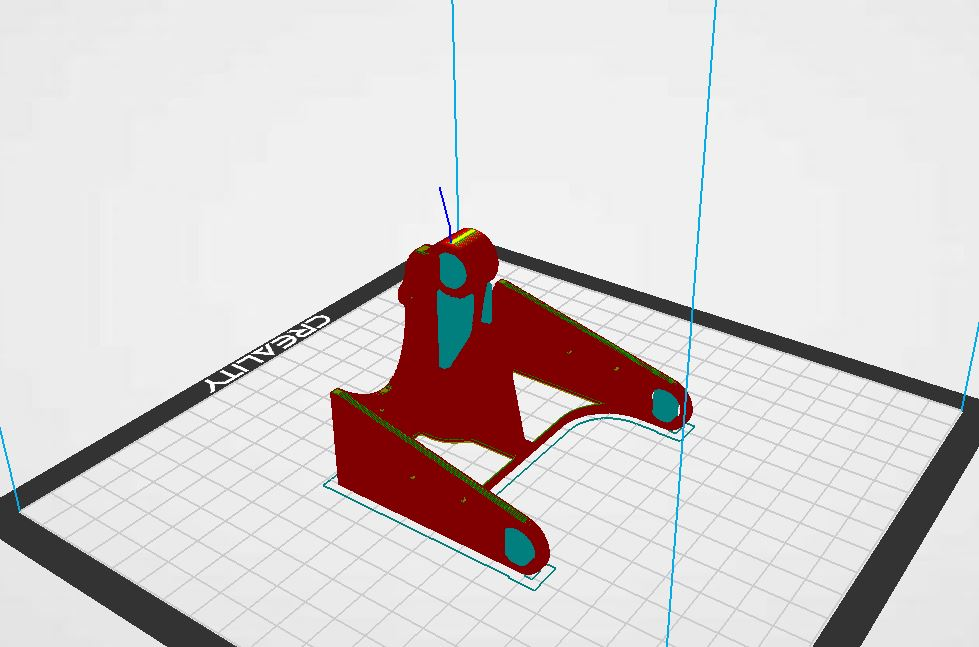
\includegraphics[width=0.95\textwidth]{Meetings/November/11-23-21/10-23-21_Hardware_Figure1 - Nathan Forrer.JPG}
  \caption{The abnormal intake shape before printing}
  \label{fig:pic1}
\end{minipage}%
\hfill%
\begin{minipage}[b]{.48\textwidth}
  \centering
  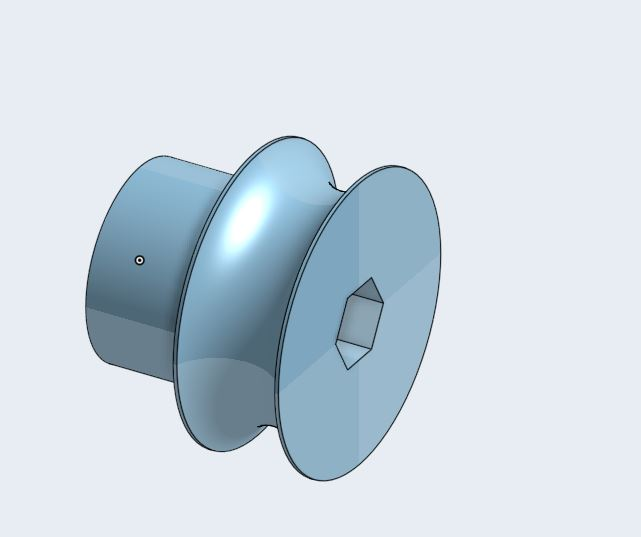
\includegraphics[width=0.95\textwidth]{Meetings/November/11-23-21/10-23-21_Hardware_Figure2 - Nathan Forrer.JPG}
  \caption{Our new pulleys with modified diameters}
  \label{fig:pic2}
\end{minipage}
\end{figure}

\begin{figure}[htp]
\centering
\includegraphics[width=0.95\textwidth, angle=0]{Meetings/November/11-23-21/10-23-21_Hardware_Figure3 - Nathan Forrer.JPG}
\caption{The finished intake piece}
\label{fig:pic3}
\end{figure}


\whatsnext{
\begin{itemize}
    \item Put 3d printed parts together
    \item Test roller intake

\end{itemize} 
}

